\documentclass[11pt, a4paper]{article}

% --- 基础宏包 ---
\usepackage[UTF8]{ctex} % 支持中文排版
\usepackage{geometry}   % 页边距设置
\usepackage{graphicx}   % 导入图片
\usepackage{amsmath, amsfonts, amssymb}
\usepackage{xcolor}     % 颜色支持
\usepackage{tocloft}    % 极方便地控制目录格式
\usepackage[hidelinks]{hyperref}   % 目录超链接（隐藏红框）
\usepackage{listings}
\usepackage{subcaption} % 提供 subfigure 环境
\usepackage{float}      % 提供 [H] 强制放置选项
\usepackage{enumitem}   % 提供 itemize 自定义格式
\usepackage{newunicodechar} % 处理 Unicode 字符映射

% Unicode 字符映射 (避免 cmr10 字体缺失报错)
% 注意: ×, “, ” 已由 ctex 定义，此处仅定义圈号数字
\newunicodechar{①}{1.}
\newunicodechar{②}{2.}
\newunicodechar{③}{3.}

% --- 页面边距设置 ---
\geometry{left=2.5cm, right=2.5cm, top=3.0cm, bottom=3.0cm}

% 全局设置风格（可选）
\lstset{
  basicstyle       = \ttfamily\small,     % 代码字体
  keywordstyle     = \color{blue},        % 关键词颜色
  commentstyle     = \color{gray},        % 注释颜色
  stringstyle      = \color{red},         % 字符串颜色
  numbers          = left,                % 左侧行号
  numberstyle      = \tiny\color{gray},   % 行号样式
  frame            = single,              % 加单线边框
  breaklines       = true,                % 自动换行
  showstringspaces = false                % 不显示空格符号
}

% --- 颜色定义 (浙江大学求是蓝) ---
\definecolor{zjublue}{RGB}{0, 63, 137}

% --- 目录样式微调 (tocloft 宏包设置) ---
\renewcommand{\contentsname}{Contents} % 将目录标题改为英文 "Contents"
\renewcommand{\cfttoctitlefont}{\normalfont\Large\bfseries} % 目录标题字号与加粗
\renewcommand{\cftsecleader}{\cftdotfill{\cftdotsep}} % 让 Section（一级标题）也使用虚线连接页码
\renewcommand{\cftsecfont}{\normalfont} % 目录中 section 字体（不加粗，与图片一致）
\renewcommand{\cftsecpagefont}{\normalfont} % 目录中 section 页码字体

\begin{document}

% =========================================================================
%                               封面开始
% =========================================================================
\begin{titlepage}
    \centering
    \thispagestyle{empty} % 封面不显示页码
    
    \vspace*{1.0cm}
    
    % 1. 浙江大学艺术字校名 (如果没有图片，会显示占位红框)
    \makebox[\textwidth][c]{
        
\includegraphics[width=13cm]{zju_name.png}
}
    
    \vspace{0.8cm}
    
    % 2. 浙江大学求是鹰 Logo
    \makebox[\textwidth][c]{
        
\includegraphics[width=5cm]{zju_logo.png}
    }
    
    \vspace{2.0cm}
    
    % 3. 报告标题
    {\fontsize{22pt}{22pt}\selectfont \textbf{课程设计}} \\
    \vspace{0.4cm}
    {\fontsize{26pt}{26pt}\selectfont \textbf{实 验 报 告}} \\
    
    \vfill % 自动垂直推拉空间
    
    % 4. 下方个人信息栏 (利用 tabular 和 makebox 精确对齐)
    \begin{center}
        \linespread{1.8}\selectfont % 调整行间距
        \begin{tabular}{r@{\hspace{0.5em}}l}
            {\large\makebox[5em][s]{实验名称}} & \underline{\makebox[18em][c]{\large program}} \\
            {\large\makebox[5em][s]{姓名}}     & \underline{\makebox[18em][c]{\large sunny}} \\
            {\large\makebox[5em][s]{学号}}     & \underline{\makebox[18em][c]{\large 5937}} \\
            {\large\makebox[5em][s]{实验日期}} & \underline{\makebox[18em][c]{\large 2006.08.10}} \\
            {\large\makebox[5em][s]{指导老师}} & \underline{\makebox[18em][c]{\large prof.}} \\
        \end{tabular}
    \end{center}
    
    \vspace*{1.0cm}
\end{titlepage}

\newpage

% =========================================================================
%                               目录页
% =========================================================================
\pagenumbering{Roman} % 目录页使用罗马数字页码（符合规范，不需要可删去）
\tableofcontents
\newpage

\pagenumbering{arabic} % 正文开始使用阿拉伯数字页码重新计数
% =========================================================================
%                               正文开始
% =========================================================================


\begin{abstract}
本课程设计围绕...展开研究，...
\begin{center}
Abstract
\end{center}

This course design focuses on the research of ...
\vspace{\baselineskip}
\par\textbf{关键词：} ...\\
\par\textbf{Keywords:} ...
\end{abstract}

\newpage

% =========================================================================
\section{引言}
% =========================================================================
\subsection{...的研究背景}
随着数字图像处理技术和计算机视觉技术的快速发展...
\subsection{传统处理方法的局限性}
...
\subsection{本课题研究内容与研究路线}
本课程设计以...为研究对象，首先分析...

% =========================================================================
\section{算法原理与数学建模}
\subsection{理论基础}
...
% =========================================================================
\subsection{数学模型}
...
\subsubsection{something...}

...

\subsubsection{something else...}

...

\subsection{算法流程}

本课程设计的整体算法流程如下：

\begin{enumerate}
\item first...；
\item sec...；
\item third...；
\item forth...；
\item fifth...；
\item more...
\end{enumerate}

整个算法充分体现了...
% =========================================================================
\section{系统实现与开发环境}
% =========================================================================
\subsection{环境搭建与工具链}
列出开发环境：for example ,Python 3.x, NumPy, OpenCV, Matplotlib 库的作用。

\subsection{系统总体设计流程}
\begin{figure}[htbp]
    \centering
    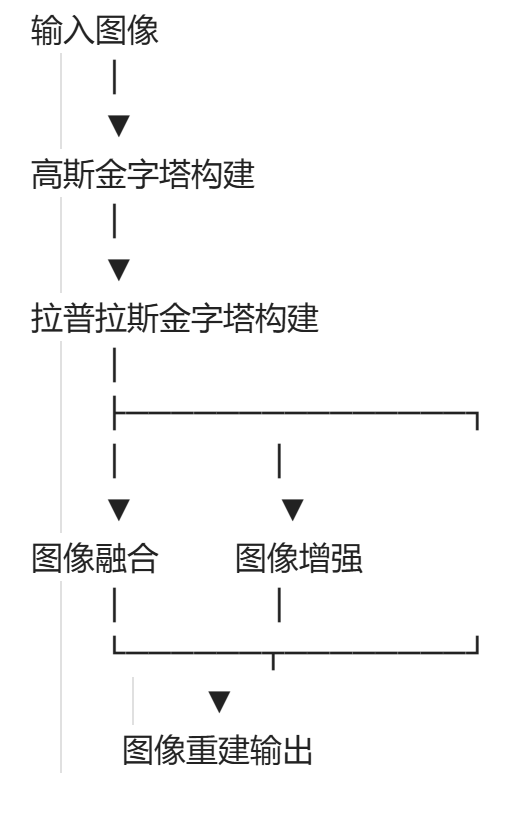
\includegraphics[width=0.3\textwidth]{./11.png} % 此处{}内请改成你自己的图片路径
    \caption{流程图}
\end{figure}

\subsection{软件模块设计与核心代码结构}
下面介绍自定义编写的 core functions 及其接口设计：
\subsubsection{first function}

\textbf{功能：}

构建...

\textbf{输入：}
\begin{itemize}
    \item \textbf{sth.}：...
    \item \textbf{sth.}：...
\end{itemize}

\textbf{输出：}
\begin{itemize}
    \item \textbf{sth.}：...
\end{itemize}

\textbf{流程：}
\begin{enumerate}
    \item firth step...
    \item second step...
    \item third step...
    \item forth step...
    \item more...
\end{enumerate}

% 下面的代码块请改成你自己的
\begin{lstlisting}   
def build_gaussian_pyramid(img, levels=4):
    pyramid = []
    current = img.astype(np.float32) if img.dtype != np.float32 else img.copy()
    pyramid.append(current)
    for _ in range(levels):
        blurred = _gaussian_blur(current)
        down = _downsample(blurred)
        pyramid.append(down)
        current = down
    return pyramid
\end{lstlisting}

% 若还有函数可以继续添加，例如：subsubsection{second function}...

% =========================================================================
\section{实验结果与仿真验证}
% =========================================================================
\subsection{...精度验证}

本实验旨在验证...的正确性。理论上，...

为了定量评价...质量，采用...作为评价指标。其中...

以下为误差图像展示。

\subsubsection{灰度重建测试效果}

% 下面是并排展示两张图片的代码

\begin{figure}[H]
    \centering
    \begin{subfigure}{0.4\textwidth}  % 可以在这里修改图片宽度大小
        \centering
        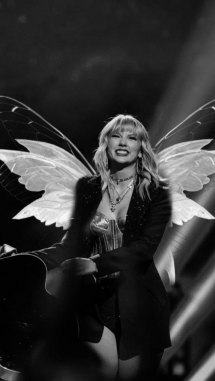
\includegraphics[width=\textwidth]{./Figure_1-img0.png} % 此处{}内请改成你自己的图片路径
        \caption{1}
        \label{fig:gray-recon-a}
    \end{subfigure}
    \hfill  % 撑开间距，也可用 \quad 或 \qquad
    \begin{subfigure}{0.4\textwidth}
        \centering
        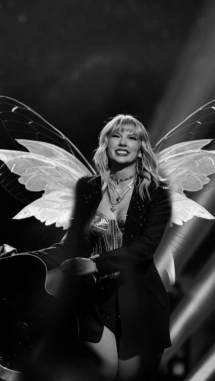
\includegraphics[width=\textwidth]{./Figure_1-img1.png} % 此处{}内请改成你自己的图片路径
        \caption{2}
        \label{fig:gray-recon-b}
    \end{subfigure}
    \caption{测试效果}
    \label{fig:gray-recon}
\end{figure}

% 下面是一组四张图片的展示代码

\begin{figure}[H]
    \centering
    % 第一排：图1 和 图2
    \begin{subfigure}{0.4\textwidth}
        \centering
        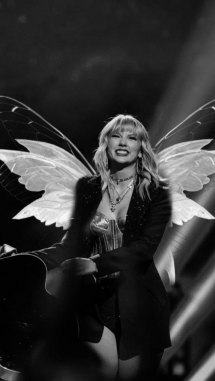
\includegraphics[width=\textwidth]{./Figure_1-img2.png}% 此处{}内请改成你自己的图片路径
        \caption{3}
        \label{fig:gray-pyr0}
    \end{subfigure}
    \hfill
    \begin{subfigure}{0.4\textwidth}
        \centering
        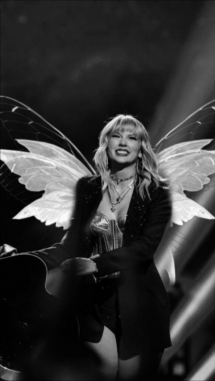
\includegraphics[width=\textwidth]{./Figure_1-img3.png}% 此处{}内请改成你自己的图片路径
        \caption{4}
        \label{fig:gray-pyr1}
    \end{subfigure}

    \par\bigskip  % 换行并留竖直间距（也可用 \vspace{1cm}）

    % 第二排：图3 和 图4
    \begin{subfigure}{0.4\textwidth}
        \centering
        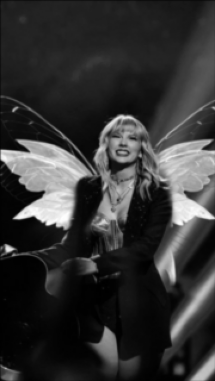
\includegraphics[width=\textwidth]{./Figure_1-img4.png}% 此处{}内请改成你自己的图片路径
        \caption{5}
        \label{fig:gray-pyr2}
    \end{subfigure}
    \hfill
    \begin{subfigure}{0.4\textwidth}
        \centering
        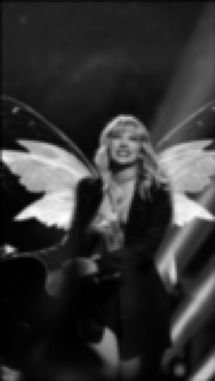
\includegraphics[width=\textwidth]{./Figure_1-img5.png}% 此处{}内请改成你自己的图片路径
        \caption{6}
        \label{fig:gray-pyr3}
    \end{subfigure}

    \caption{重建过程}% 这组图片的名称
    \label{fig:gray-pyramid}
\end{figure}

\textbf{结果分析：}
\\  由上述图可以看出，...
进一步观察误差热图可以发现，...

实验结果说明，本文实现的...具有良好的...,能够...

% 其他的测试结果展示也可以继续在下面添加，for example:\subsubsection{...}




\subsection{参数灵敏度分析}
实验测试不同的...以及不同频段的...对...的影响
我将通过三个定量指标来比较，它们分别是：
% 这里的指标请自行修改
\\1. RMSE：表示增强图与原图的均方根误差，越小表示越接近原图\\
2. PSNR：表示增强图与原图的峰值信噪比，越大表示增强效果越好、失真越小\\
3. Grad：表示增强图的图像锐度，越大表示增强后的图像细节越丰富\\
以下是四组参数的对比图：

\begin{figure}[H]
    \centering
% 第一排：图2 和 图3
    \begin{subfigure}{0.3\textwidth}
        \centering
        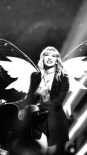
\includegraphics[width=\textwidth]{./Figure_4-img1.png}
        \caption{第一组增强结果(\texttt{levels}=3, \texttt{gain\_high}=2.0, \texttt{gain\_mid}=2.0, \texttt{gain\_low}=2.0)}% 此处{}内请改成你自己的图片路径
        \label{fig:enhance-g1}
    \end{subfigure}
    \hfill
    \begin{subfigure}{0.3\textwidth}
        \centering
        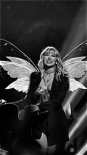
\includegraphics[width=\textwidth]{./Figure_4-img2.png}
        \caption{第二组增强结果(\texttt{levels}=4, \texttt{gain\_high}=2.8, \texttt{gain\_mid}=1.0, \texttt{gain\_low}=1.0)}% 此处{}内请改成你自己的图片路径
        \label{fig:enhance-g2}
    \end{subfigure}
\end{figure}



对比结果汇总如下：

%插入左对齐的图像的代码如下：

\begin{figure}[H]
    % 去掉 \centering，整个 figure 左对齐
    \raggedright
    % 第二张图（下方）
    \begin{subfigure}{0.7\textwidth}
        \centering
        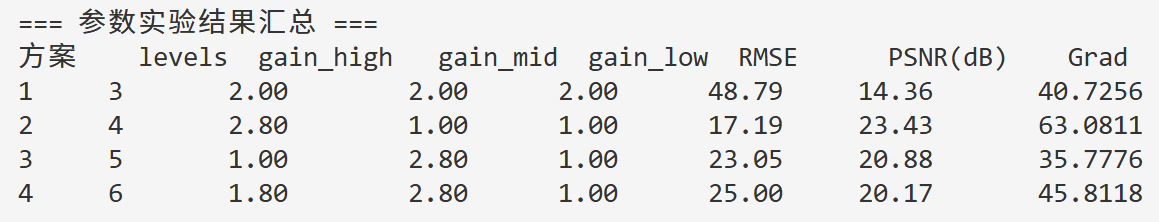
\includegraphics[width=\textwidth]{./4-2.png}% 此处{}内请改成你自己的图片路径
        \caption{结果汇总表}
        \label{fig:enhance-table}
    \end{subfigure}

    \caption{多尺度细节增强实验结果对比}
    \label{fig:enhance-summary}
\end{figure}

\textbf{参数影响分析}
\\由实验结果可以发现，不同...以及不同...会对增强效果产生明显影响。
...
\\综合RMSE、PSNR及Gradient三个评价指标可以发现，...
\subsection{性能评估}
这里我对三种方案进行了对比，方案A即为我的全手写实现方案，方案 B 的重建部分仍然是手写的，但是下采样高斯模糊用了 OpenCV，而方案三是完全使用OpenCV的结果。\\
对比结果见下图：\\

% 插入单张图片

\begin{figure}[H]
    \centering
    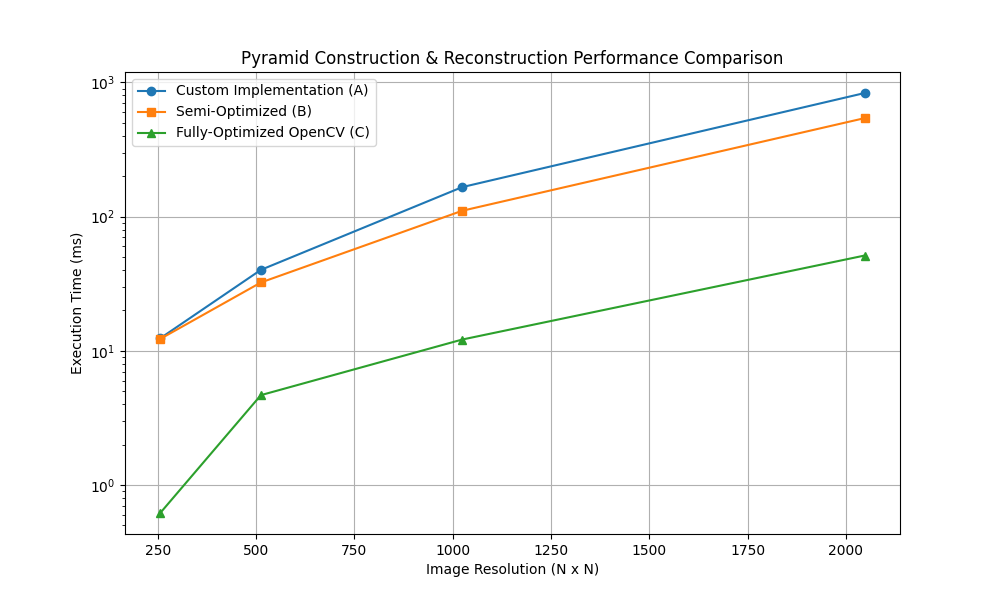
\includegraphics[width=0.9\textwidth]{./performance_comparison.png}
    \caption{性能差距对比表（方案对比）}
    \label{fig:perf-comparison}
\end{figure}



\textbf{原因分析}
...

\textbf{总结分析}
\\综合实验结果可以看出，...
% =========================================================================
\section{结论}
% =========================================================================
本课程设计以...为研究对象，系统完成了...,有效改善了...


% =========================================================================
\section*{参考文献}
% =========================================================================
\addcontentsline{toc}{section}{参考文献}

\begin{description}
\item[{[1]}] ...

\item[{[2]}] ...

\item[{[3]}] more...
\end{description}

\end{document}
